\chapter{Engineering}
We are normally shocked at the marvelous pay top engineers earn. It almost feels like they know something that the normal population doesn't. Is it math? no. If you are reading this chapter towards the end, you probably are better at math than most engineers.\\
Is it coding? Not really. A lot of coders just copy and hack code from google.\\
Is it that they are smarter than the rest of the population? Based on my conversations and IQ tests, Negitive.\\
So why? because they have \cancel{learnt} mastered the art of engineering. Engineering is finding the answer to a problem without solving it. It’s the art of problem solving minus the solving part, we don't do that here. It is finding the answer with less effort than it would take us if we did the problem “properly”.\\
While engineering is a useful skill, it is by no means replacement for learning math. Remember the high ball engineers we talked about can still code if google stopped working. In fact, it will be them who will get it to start working again. They can solve the problem, but for efficiency use such methods.\\
It shouldn’t be satisfying to get an answer with engineering. Engineering a problem is like taking out a loan, that you need to repay with learning the actual solution to the problem. THIS CHAPTER IS NOT FOR PEOPLE WHO ARE YET TO SOLVE THE REST OF THE BOOK.\\
That is a disclaimer, as if misunderstood this chapter can do more harm than good, and don’t say I didn’t warn you.\\
\section{Abuse of Degree of Freedom}
\begin{example}
(PMO 2019) In triangle $ABC$, $D$ and $E$ are points on sides $AB$ and $AC$ respectively, such that $BE$ is perpendicular to $CD$. Let $X$ be a point inside the triangle such that $\angle XBC = \angle EBA$ and $\angle XCB = \angle DCA$. If $\angle A = 54^\circ$, what is the measure of $\angle EXD$?
\end{example}
While I assume you can already solve this geometrically, the engineering solution comes by noticind that the question is general, hence if $D$ was placed right on $A$, and therefore $BE \perp AC$ and therefore $X$ is placed right on $B$ making this a simple angle sum.
\begin{figure} [h]
    \centering
    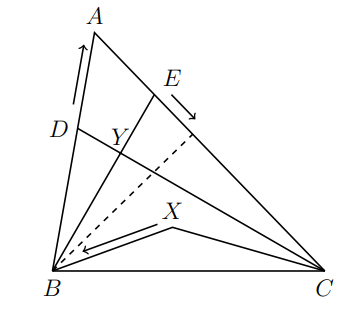
\includegraphics[width=0.5\linewidth]{Photos/PMO 2019 III 4.png}
    \caption{The question diagram as we engineer it out of existence}
    
\end{figure}
\begin{example}
    Let $S$ be any point within a rectangle $ABCD$. On $AS$, a square $ASRF$ is described and $E$ is a point on $AB$ such that $AE = AD$. The value of $((\frac{AF+ES}{FD+AS})^{\frac{1}{2}}+3)^{\frac{1}{2}}$
\end{example}
This question dies a sad death by simply letting $E=S$\\
